% Ta dokument je bil ustvarjen na osnovi predloge za poročila o domačih
% nalogah, katere nosilec je Blaž Zupan in je dostopna na spletni učilnici
% predmeta UOZP.

\documentclass[a4paper,11pt,titlepage]{article}
\usepackage{a4wide}
\usepackage{fullpage}
\usepackage[utf8x]{inputenc}
\usepackage[slovene]{babel}
\selectlanguage{slovene}
\usepackage[toc,page]{appendix}
\usepackage[pdftex]{graphicx} % za slike
\usepackage{setspace}
\usepackage{color}
\definecolor{light-gray}{gray}{0.95}
\usepackage{listings} % za vključevanje kode
\usepackage{hyperref}
\usepackage{titlesec}
\usepackage{amsmath}
\usepackage{amsthm}

\renewcommand{\baselinestretch}{1.1} % za boljšo berljivost večji razmak
\renewcommand{\appendixpagename}{\normalfont\Large\bfseries{Priloge}}

\lstset{ % nastavitve za izpis kode
language=Python,
basicstyle=\footnotesize,
basicstyle=\ttfamily\footnotesize\setstretch{1},
backgroundcolor=\color{light-gray},
}

\title{Strojno učenje za boljšo povečavo slik}
\author{Blaž Rojc}
\date{\today}

\begin{document}

\maketitle

\section{Uvod}

Današnja fotografska oprema, od profesionalnih fotoaparatov do pametnih telefonov, je zmožna zajemati slike v visokih ločljivostih.
Ker pogosto polna ločljivost slike ni potrebna, se večina slik pred shranjevanjem ali pošiljanjem zmanjša.
To samo po sebi ne bi bil problem, če bi se za spreminjanje velikosti uporabljali algoritmi, ki bi skušali čim bolj ohraniti kvaliteto slike.
Ampak zaradi minimizacije stroškov procesiranja in shranjevanja veliko aplikacij uporablja linearno interpolacijo, ki na račun kvalitete omogoča zelo
	hitro spreminjanje velikost slike.

S ciljem boljše povečave slik sem ustvaril konvolucijsko nevronsko mrežo, ki vzame linearno interpolirano, v vsako dimenzijo štirikrat povečano sliko
	in vrne izboljšano verzijo z manj artifakti povečave.
V tem besedilu bom predstavil delovanje nevronske mreže, njeno obliko, programsko okolje, ki sem ga uporabil, in množico slik, uporabljeno
	pri treniranju in preizkušanju mreže.

Pri načrtovanju mreže sem se usmerjal po raziskavah s podobnim namenom. \cite{intel1, intel2, intel3}
V večini primerov je šlo za večslojne nevronske mreže, jaz sem se pa omejil na en sloj s knovolucijo.

Rezultati so sprejemljivi, mreža je zmožna očitno izboljšati kvaliteto slike v primerjavi z linearno interpolacijo samo.

\section{Definicije}

V tem besedilu so večkrat uporabljeni izrazi \emph{konvolucija}, \emph{aktivacijska funkcija} in \emph{konvolucijska nevronska mreža}.
Definirajmo jih.

\subsection{Konvolucija}

\emph{Konvolucija} \cite{torch_conv2d} je računska operacija, podana s formulo

\begin{equation*}
\text{izhod}(C_{izhod_j}) =
	\text{odmik}(C_{izhod_j}) + \sum_{\substack{C_{vhod_i} \\ \in C_{vhod}}} \text{utež}(C_{izhod_j}, C_{vhod_i}) \star \text{vhod}(C_{vhod_i}) \text{,}
\end{equation*}

kjer sta $C_{izhod_j}$ in $C_{vhod_i}$ barvna kanala slike, $C_{vhod} = C_{izhod} = (\text{rdeč}, \text{zelen}, \text{moder})$,
	oznaka $\star$ pa označuje \emph{diskretno korelacijo}, podano s formulo

\begin{equation*}
(f\star g) (n) = \sum_{m = - \infty}^{\infty} \overline{f(m)} \cdot g(m + n) \text{.}
\end{equation*}

Oznaka $\overline{f}$ nakazuje, da gre za kompleksno konjugiranko $f$, ampak ker so vsi vhodi, uteži in odmiki realna števila,
	uporabljamo pa le operaciji seštevanja in množenja, velja $\overline{f} = f$ in enačbo lahko zapišemo v obliki

\begin{equation*}
(f\star g) (n) = \sum_{m = - \infty}^{\infty} f(m) \cdot g(m + n) \text{.}
\end{equation*}

Vemo, da ima funkcija uteži končno definicijsko območje, zato se omejimo le na $k$ členov:

\begin{equation*}
(f\star g) (n) = \sum_{m = 0}^{k - 1} f(m) \cdot g(m + n)
\end{equation*}

Število k imenujemo \emph{jedro konvolucije}.

Slike so dvodimenzionalni objekti, v računalniku predstavljeni kot trojica dvodimenzionalnih matrik - vsaka predstavlja intenzivnosti
	enega izmed treh barvnih kanalov.\footnote{\url{https://en.wikipedia.org/wiki/Raster\_graphics}}
Torej moramo pojem konvolucije razširiti na dve dimenziji:

\begin{equation*}
(f\star g) (x, y) = \sum_{m, n = 0}^{k - 1} f(m, n) \cdot g(x + m, y + n)
\end{equation*}

Vstavimo sedaj to formulo v definicijo konvolucije in računajmo za točko $(x, y)$:

\begin{multline*}
\text{izhod}(C_{izhod_j}, x, y) = \\
	\text{odmik}(C_{izhod_j}, x, y) + \sum_{\substack{C_{vhod_i} \\ \in C_{vhod}}} \sum_{m, n = 0}^{k - 1}
	\text{utež}(C_{izhod_j}, C_{vhod_i}, m, n) \cdot \text{vhod}(C_{vhod_i}, x + m, y + n)
\end{multline*}

Opazimo: `vhod', `izhod' in `odmik' so trodimenzionalne podatkovne strukture, `utež' pa kar štiridimenzionalna.
Take strukture imenujemo \emph{tenzorji}.

\subsection{Aktivacijska funkcija}

Izraz \emph{aktivacijska funkcija} označuje funkcijo, ki izhodno vrednost sloja mreže preslika v vrednost v želenem območju.\cite{activation_func_1}
V globokih nevronskih mrežah se aktivacijske funkcije uporabljajo za vnos nelinearnosti,
	ki omogoča smiselno komponiranje operacij.\cite{activation_func_2}

Nekaj primerov aktivacijskih funkcij predstavljajo usmerjena linearna enota (ReLU):
\begin{equation*} 
f(x) = \begin{cases}
	0 & \text{za } x < 0 \\
	x & \text{za } x \ge 0
\end{cases}
\end{equation*}
sigmoid:
\begin{equation*} 
f(x) = \frac{1}{1 + e^{-x}}
\end{equation*}
in binarna stopnica:
\begin{equation*} 
f(x) = \begin{cases}
	0 & \text{za } x < 0 \\
	1 & \text{za } x \ge 0
\end{cases}
\end{equation*}

\subsection{Nevronska mreža}

\begin{figure}[htbp]
\begin{center}
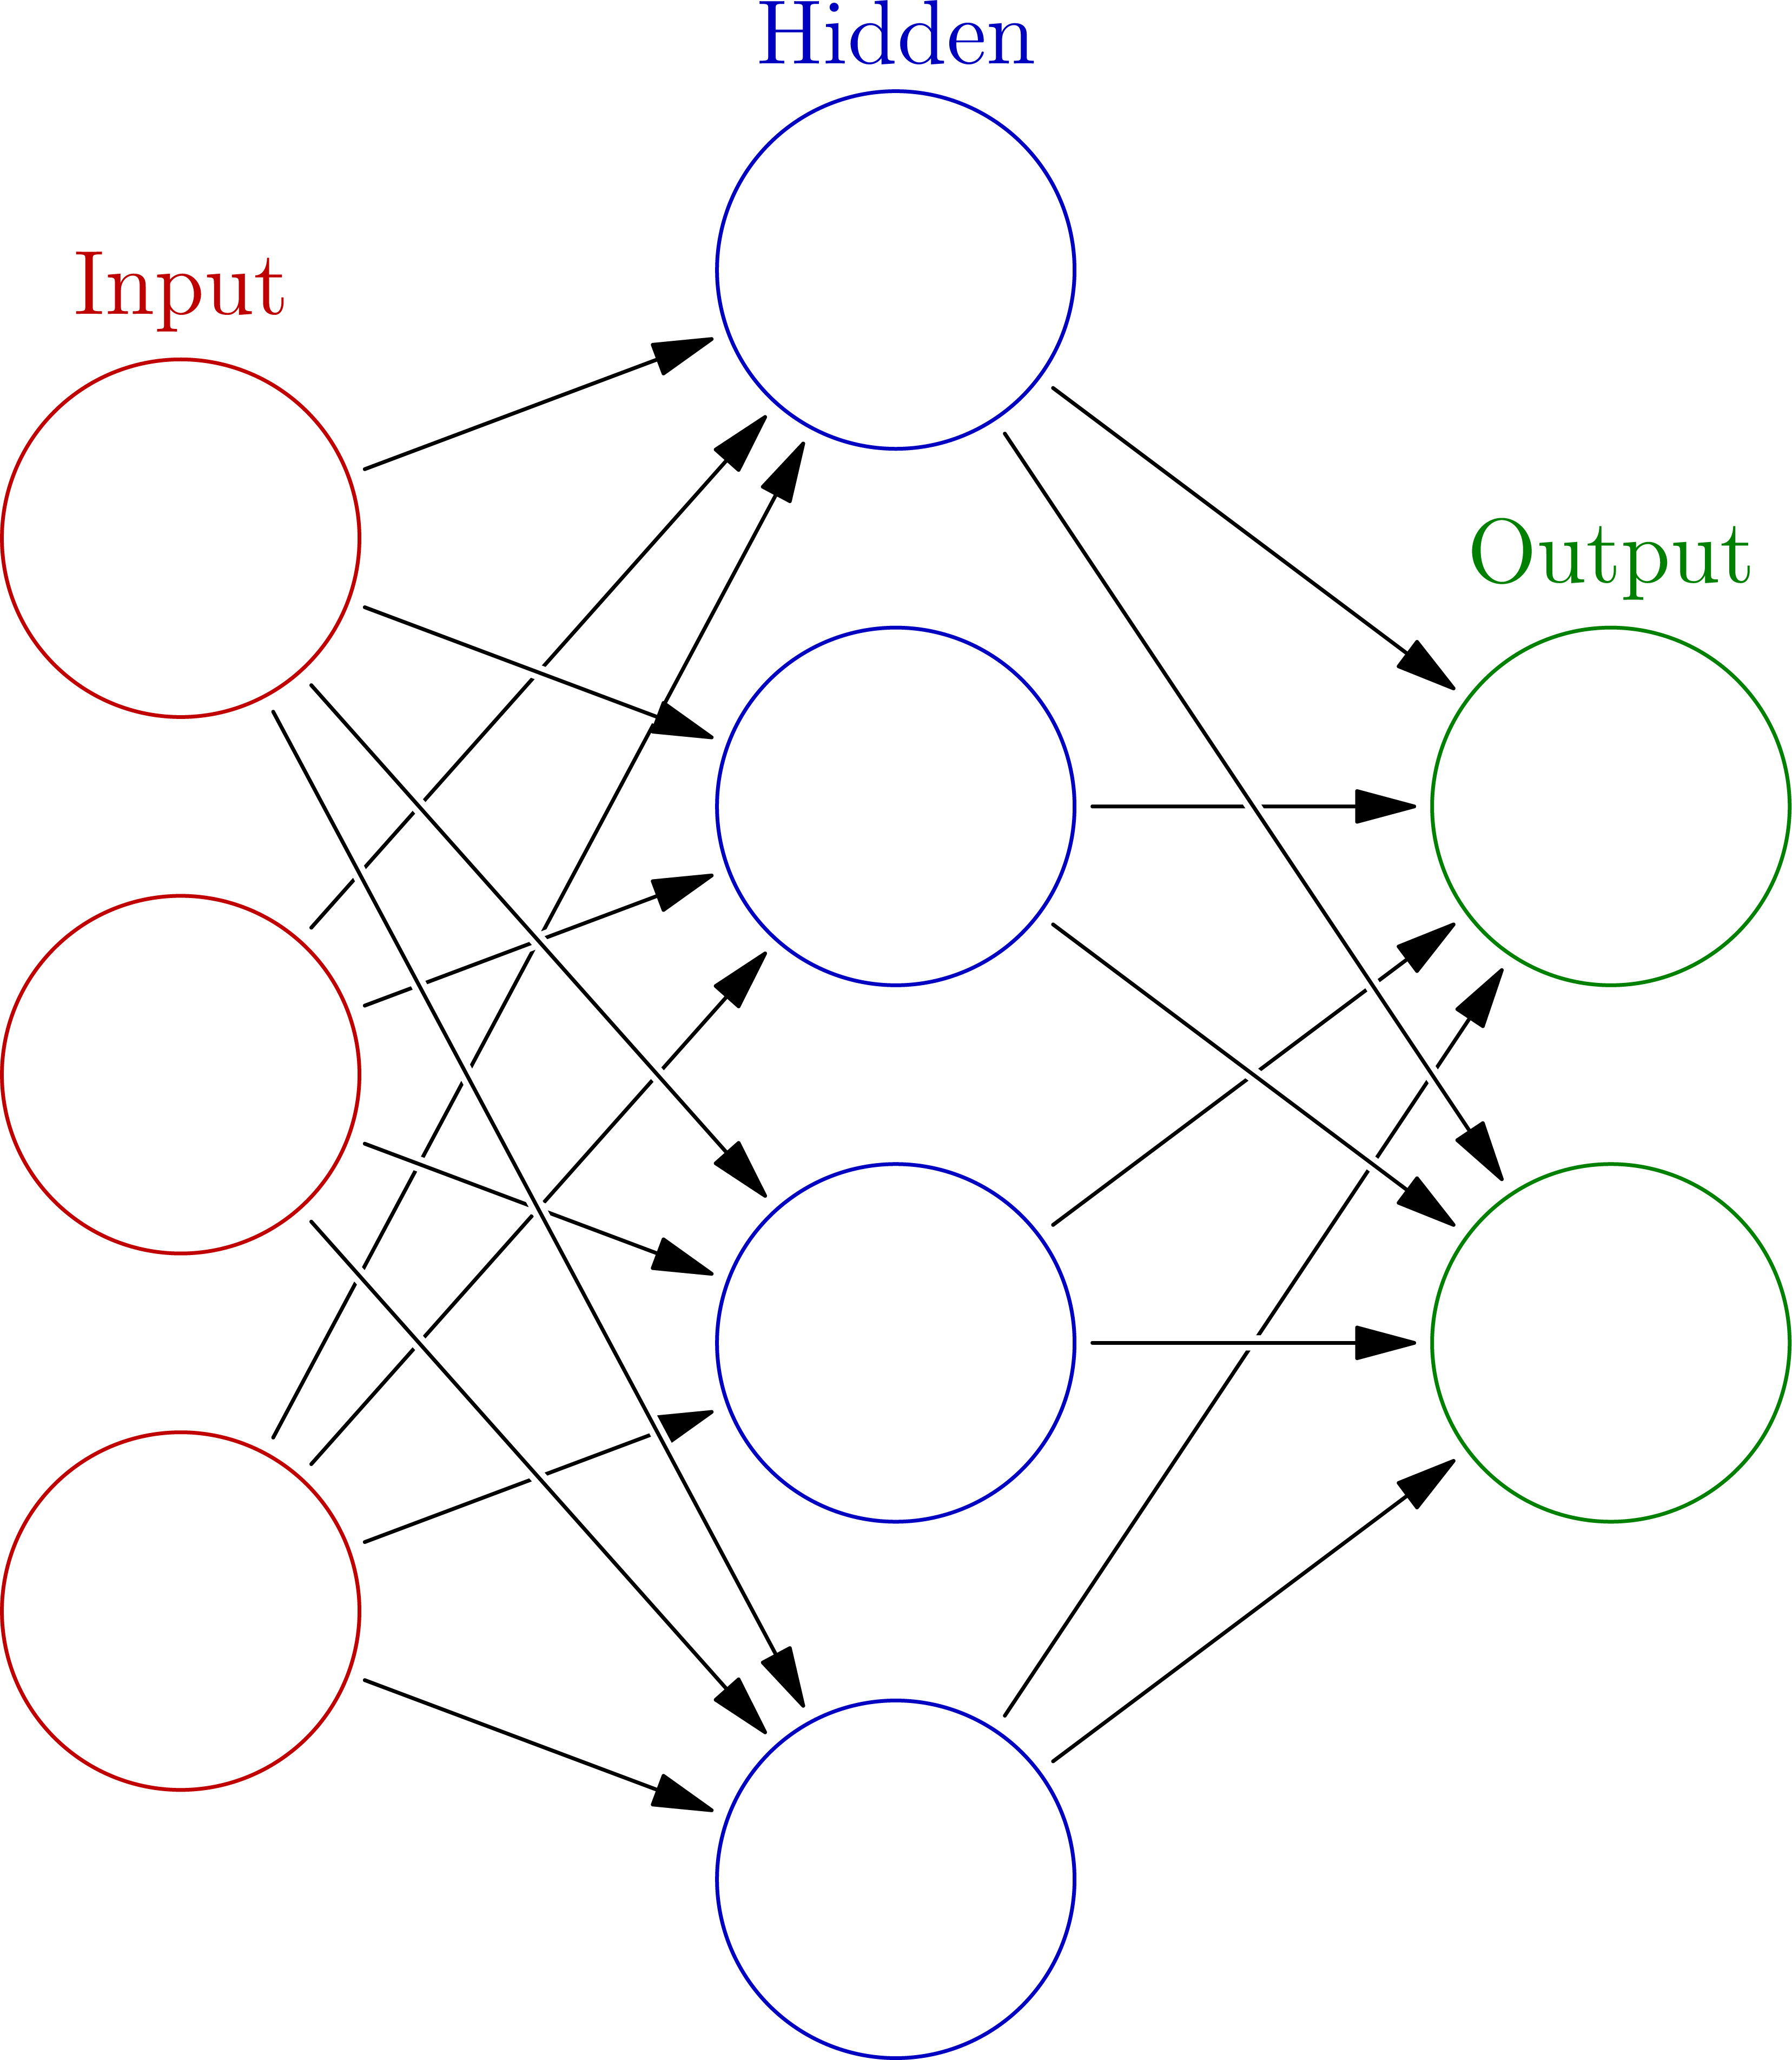
\includegraphics[scale=0.25]{neural_network.png}
\caption{Primer nevronske mreže. vir:
	\href{https://en.wikipedia.org/wiki/Artificial\_neural\_network\#/media/File:Colored\_neural\_network.svg}{Wikipedia}}
\label{slika1}
\end{center}
\end{figure}
\emph{Nevronska mreža} je omrežje povezanih nevronov ali vozlišč.\cite{ann_def_1}
Njena oblika se zgleduje po strukturi živalskih možganov.\cite{ann_def_2}
Podobno se tudi ``uči'': Za vsak učni primer se prilagodi glede na razliko med njenim in ciljnim izhodom.

Prednost nevronske mreže v primerjavi s standardnimi algoritmi je, da za gradnjo mreže postopka iskanja rešitve ni potrebno točno definirati.
Na razpolago moramo imeti le dovolj velik nabor parov vhodnih podatkov in pripadajočih izhodov - \emph{učno množico} - in dovolj računske moči.
Posledično lahko z njimi rešujemo probleme, ki so preveč kompleksni za direktno algoritmično reševanje ali pa algoritma sploh ne moremo definirati,
	na primer klasifikacija slik, aproksimacija težko izračunljivih funkcij, regresijska analiza \ldots

Slabost nevronske mreže je njena nenatančnost.
Večina nevronskih mrež ne doseže 100\% natančnosti, kar pomeni, da niso primerne za življenjsko kritične namene.
Poleg tega za doseganje dobrih rezultatov zahtevajo ogromne, raznolike učne množice in veliko računskega časa.\cite{ann_compute}

\subsection{Konvolucijska nevronska mreža}

\emph{Konvolucijske nevronske mreže} so eden izmed tipov usmerjenih nevronskih mrež.
Navadno so sestavljene iz več slojev, kjer so posamezni sloji konvolucije, aktivacijske funkcije, združevalne funkcije ali
	\emph{polno povezani sloji} - sloji, pri katerih je vsak nevron vhoda uteženo povezan z vsakim nevronom izhoda.
Konvolucije emulirajo odziv nevronov na lastnosti vhodnih stimulusov,\cite{cnn_conv} podobno kot ljudje bel krog na temnem ozadju zaznamo kot
	vir svetlobe.
Združevalne funkcije, kot so max$(A)$, min$(A)$ in avg$(A)$ zmanjšajo količino vmesnih podatkov, kar poenostavi proces učenja.\cite{cnn_pool}

Pravilno načrtovane konvolucijske nevronske mreže potrebujejo relativno malo preprocesnega dela, kar omogoča hiter in enostaven razvoj programov,
	ki jih uporabljajo.

\section{Oblika}

Poglejmo si obliko ustvarjene nevronske mreže (v nadaljevanju: mreža) in format vhodnih podatkov.

\subsection{Načrt mreže}

Mreža je sestavljena iz dveh slojev, in sicer ene konvolucije z jedrom velikosti $k$ ter aktivacijske funkcije pritrditve (ang. \emph{clamp}),
	definirane kot:
\begin{equation*} 
clamp(x) = \begin{cases}
	255 & \text{za } x > 255 \\
	x & \text{za } x \in [0, 255] \\
	0 & \text{za } x < 0
\end{cases}.
\end{equation*}
Tu nelinearnost aktivacijske funkcije ne igra posebne vloge, pomaga pa omejiti izhodno vrednost v dopustno območje, ki ga lahko shranimo kot 1 bajt.
Za vhod vzame povečano sliko dimenzij $(\text{širina}, \text{višina})$, vrne pa sliko dimenzij $(\text{širina} - k + 1, \text{višina} - k + 1)$.

\subsection{Oblika podatkov}

\begin{figure}[htbp]
\begin{center}
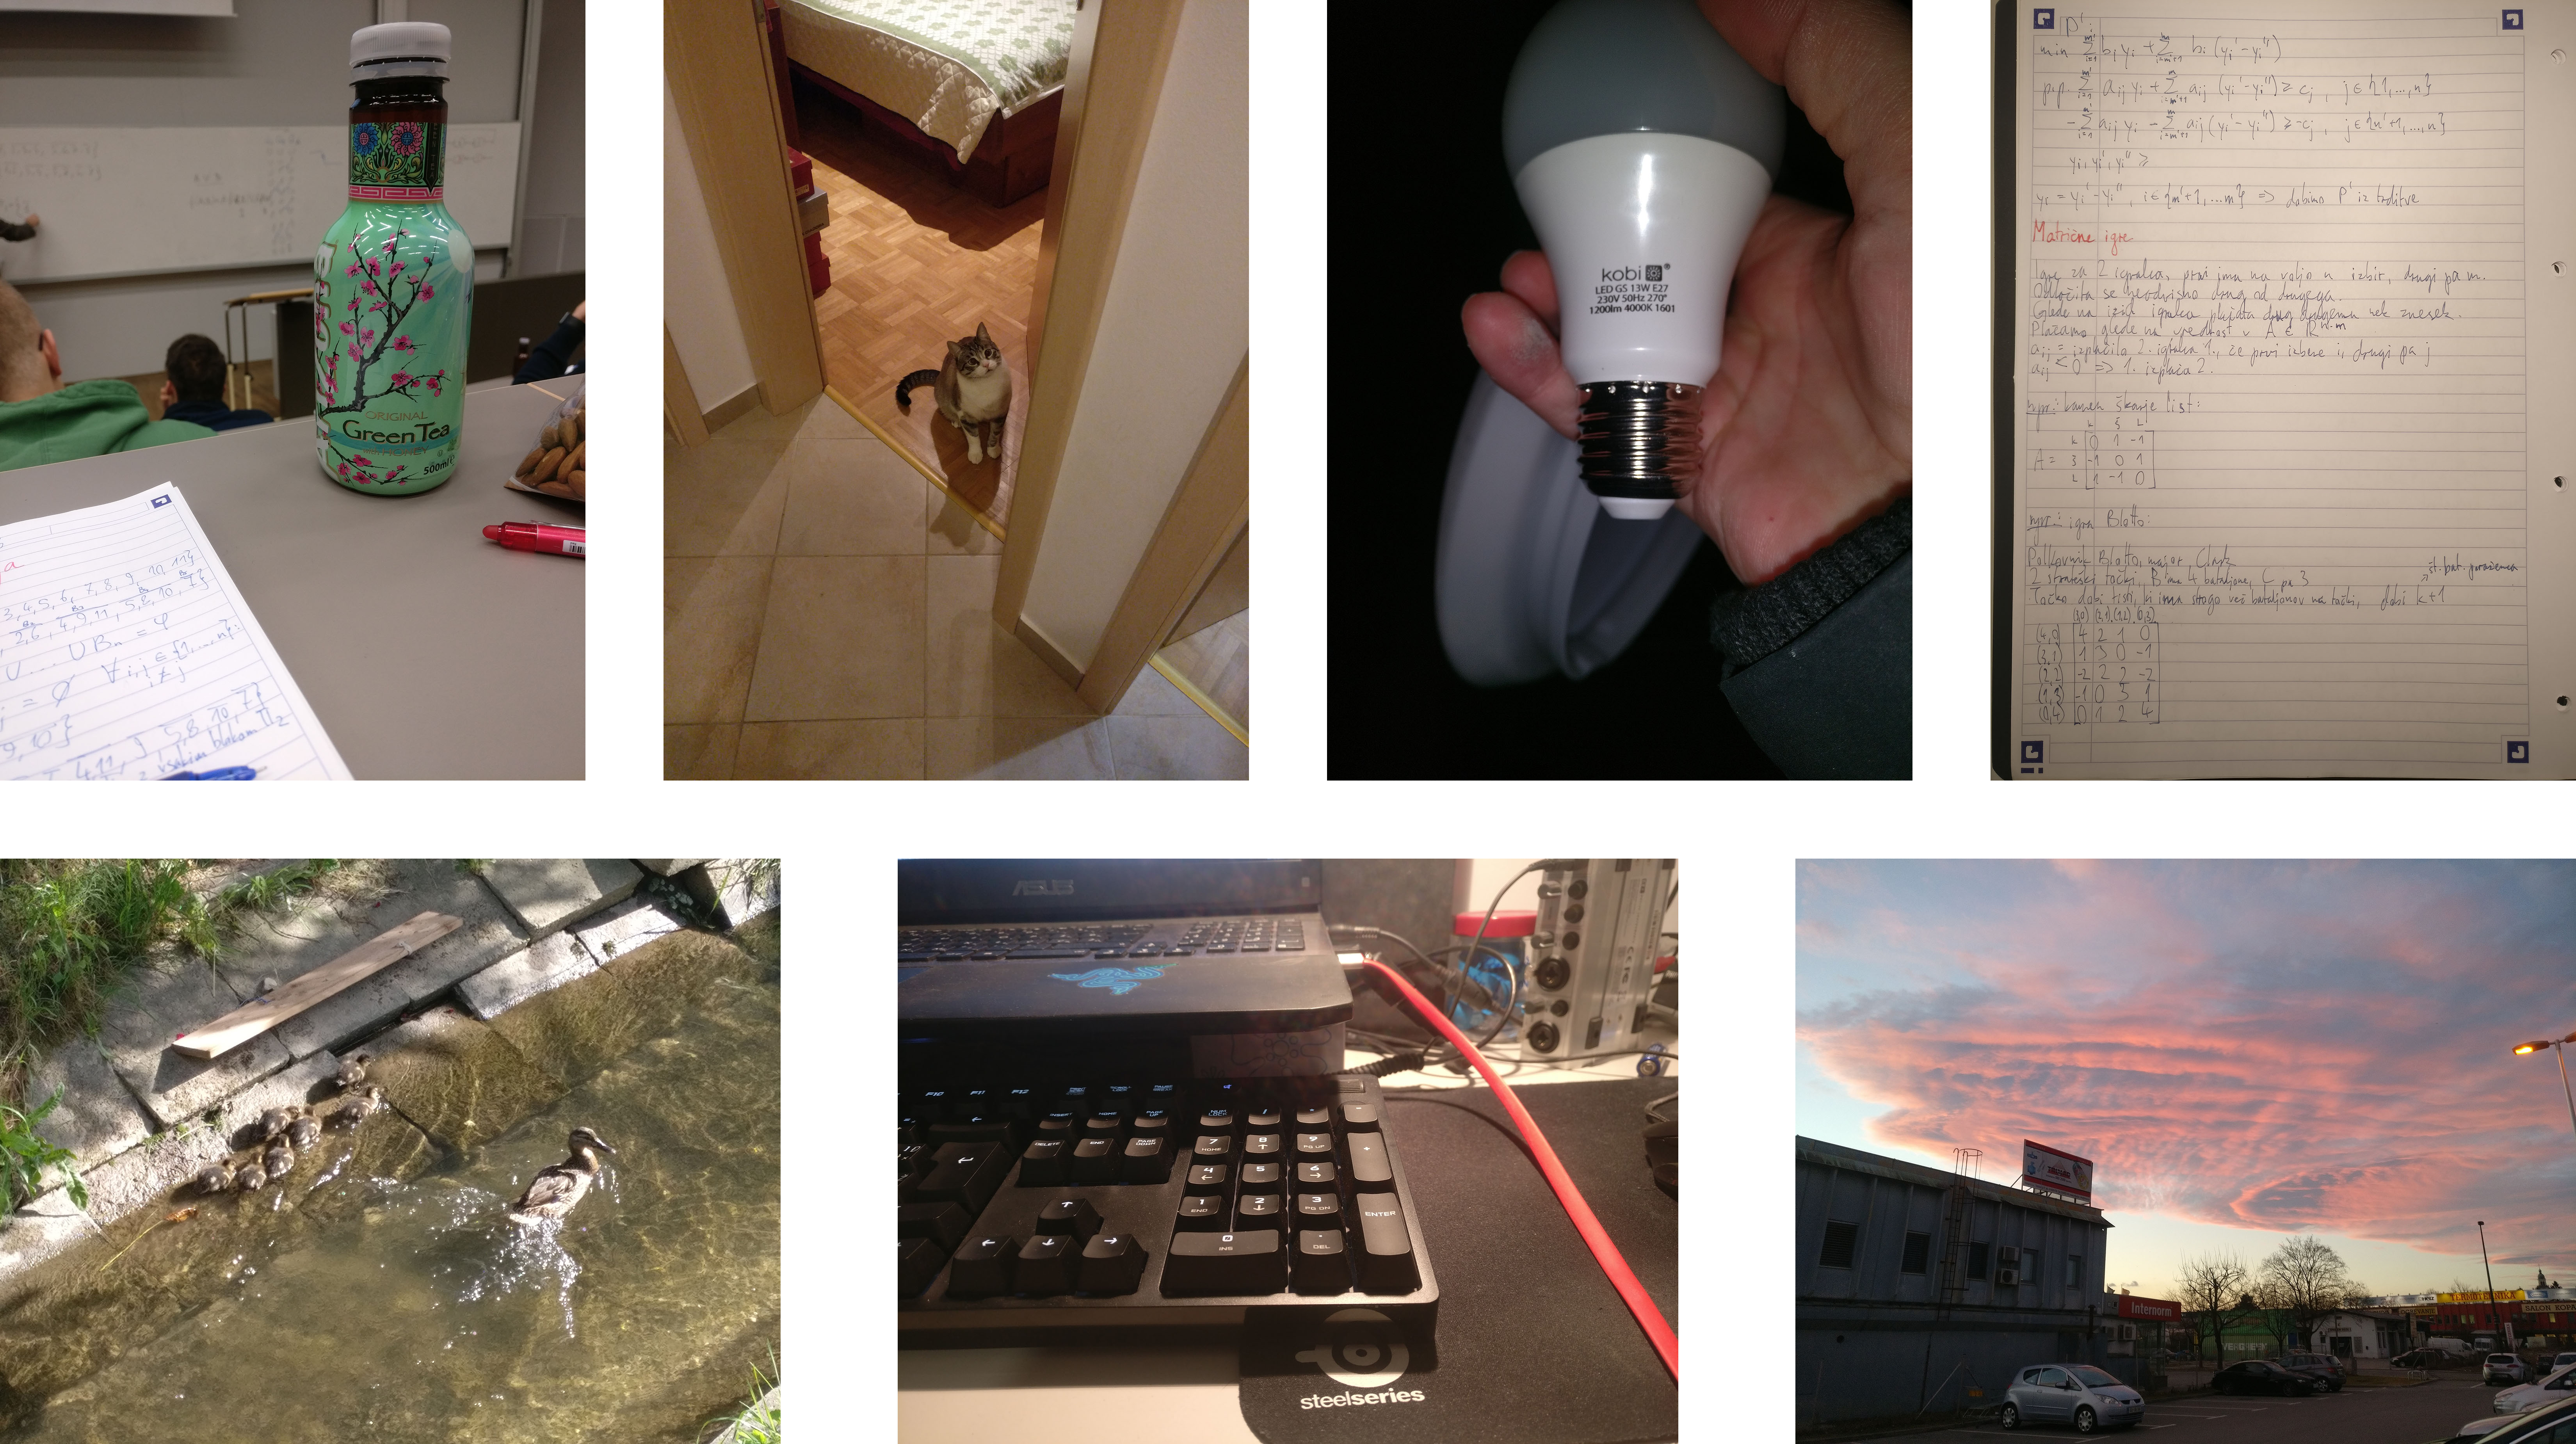
\includegraphics[scale=0.25]{picture_samples.jpg}
\caption{Primeri slik iz množice vhodnih podatkov.}
\label{slika1}
\end{center}
\end{figure}

Za množico vhodnih podatkov sem izbral 644 slik, ki sem jih naredil z mojim pametnim telefonom v obdobju zadnjih dveh let in nekaj mesecev.
Predstavljajo raznolik nabor, slikal sem ljudi, živali, naravo, zapiske, naključne predmete in še kaj.

Velikosti slik so različne, ampak večina jih je oblike (3480, 4640) ali (4640, 3480), kar predstavlja 16M pikslov.
Stisnjene so z le rahlimi izgubami, vsebujejo pa zmerno količino statičnega šuma, kar sem pred učenjem poskušal omiliti z rahlim Gaussovim filtrom.

Slike so razdeljene na dva dela.
Prvi del je učna množica 580 slik, drugi pa testna množica 64 slik.
Slike so bile razdeljene naključno, s funkcijo \texttt{random.sample} v programskem jeziku Python 3.

\section{Programsko okolje}

Mrežo sem implementiral v programskem jeziku Python 3, uporabil sem knjižnico za strojno učenje \href{https://pytorch.org/}{PyTorch}.
Ker sem hotel izvajati učenje na grafični kartici, sem namestil tudi gonilnike za platformo CUDA in knjižnico cuDNN.
Za delo s tenzorji sem uporabil knjižnico \texttt{numpy}, za delo s slikami pa knjižnico \texttt{scikit_image}.


\section{Učenje}

\section{Rezultati}


\section{Zaključek}


\begin{thebibliography}{99}

% članek na spletni strani: \bibitem{tag} Avtor. (leto). Naslov. \emph{Stran/publikacija}. [Online] Dosegljivo: \url{url}. [Dostopano \today].
% študija: \bibitem{tag} Avtor, ``Naslov''. Institucija, (št.poročila, datum).

\bibitem{intel1} Alberto V\@. (2017). An Example of a Convolutional Neural Network for Image Super-Resolution.
	\emph{Intel AI Academy} [Online]. Dosegljivo:
	\url{https://software.intel.com/en-us/articles/an-example-of-a-convolutional-neural-network-for-image-super-resolution}.
	[Dostopano \today].

\bibitem{intel2} Chao Dong \emph{et al}., ``Learning a Deep Convolutional Network for Image Super-Resolution''. The Chinese University of Hong Kong.

\bibitem{intel3} Jiwon Kim \emph{et al}., ``Accurate Image Super-Resolution Using Very Deep Convolutional Networks''.
	Seoul National University, Korea.

\bibitem{torch_conv2d} \texttt{torch.nn.Conv2d}. \url{https://pytorch.org/docs/stable/nn.html}. [Dostopano \today].

\bibitem{activation_func_1} ``What is an Activation Function?''. \url{https://deepai.org/machine-learning-glossary-and-terms/activation-function}.
	[Dostopano \today].

\bibitem{activation_func_2} Avinash Sharma V\@. (2017). Understanding Activation Functions in Neural Networks. \emph{The Theory Of Everything}.
	[Online] Dosegljivo: \url{https://medium.com/the-theory-of-everything/understanding-activation-functions-in-neural-networks-9491262884e0}.
	[Dostopano \today].

\bibitem{ann_def_1} J.~ J.~ Hopfield. (1982). Neural networks and physical systems with emergent collective computational abilities.
	\emph{Proceedings of the National Academy of Sciences of the United States of America}. [Online] Dosegljivo:
	\url{http://www.pnas.org/content/pnas/79/8/2554.full.pdf}. [Dostopano \today].

\bibitem{ann_def_2} Marcel van Gerven, Sander Bohte. (2018). Artificial Neural Networks as Models of Neural Information Processing.
	\emph{Frontiers in Computational Neuroscience}. [Online] Dosegljivo:
	\url{https://www.frontiersin.org/research-topics/4817/artificial-neural-networks-as-models-of-neural-information-processing}.
	[Dostopano \today].

\bibitem{ann_compute} Chris Edwards. (2015). \emph{Growing pains for deep learning}. Communications of the ACM. 58 (7): 14–16.

\bibitem{cnn_conv} \emph{Convolutional Neural Networks (LeNet) – DeepLearning 0.1 documentation}. DeepLearning 0.1. LISA Lab.
	[Online] Dosegljivo: \url{http://deeplearning.net/tutorial/lenet.html}. [Dostopano \today].

\bibitem{cnn_pool} Alex Krizhevsky \emph{et al}. (2012). ImageNet Classification with Deep Convolutional Neural Networks.
	\emph{NIPS 2012}. [Online] Dosegljivo: \url{http://www.image-net.org/challenges/LSVRC/2012/supervision.pdf}. [Dostopano \today].

\end{thebibliography}

\end{document}

% od predloge

\section{Uvod.}
V tem razdelku, ki naj bo kratek in naj obsega en odstavek z do 150
besed, na kratko opišeš, kaj je bil cilj naloge.

\subsection{Podatki.}
Če je naloga zasnovana tako, da vključuje analizo izbranih podatkov, v
tem razdelku opišeš, kakšni so ti podatki in navedeš nekaj osnovnih
statističnih lastnosti teh podatkov. Slednje vključujejo velikost
podatkov (na primer število primerov, število in vrsto atributov), delež
manjkajočih podatkov, opis in porazdelitev vrednosti ciljnih
spremenljivk, in podobno. Če si podatke pridobil sam, tu opišeš, na
kakšen način, kje in kako.

\section{Metode.}
Tu opišeš, na kakšen način si rešil nalogo (tehnike in metode, ki si
jih uporabil). Lahko vključiš tudi zanimiv del programske kode, ki
si jo morda pri tem razvil ali pa v poročilo dodatno vključiš sliko,
kot je na primer slika. Vse slike in tabele, ki jih
vključiš v poročilo, morajo biti navedene v besedilu oziroma se moraš
na njih sklicati.

\begin{figure}[htbp]
\begin{center}
%\includegraphics[scale=0.3]{slika-primer.png}
\caption{Vsako sliko opremi s podnapisom, ki pove, kaj slika prikazuje.}
%\label{slika1}
\end{center}
\end{figure}

V to poglavje lahko tudi vključiš kakšen metodološko zanimiv del
kode. Primer vključitve kode oziroma implementirane funkcije v
programskem jeziku Python je:

\begin{lstlisting}
def fib(n):
    if n == 0:
        return 0
    elif n == 1:
        return 1
    else:
        return fib(n-1) + fib(n-2)
\end{lstlisting}

Izris te kode je lahko sicer tudi lepši, poskušaš lahko najti še
primernejši način vključevanja kode v Pythonu oziroma v tvojem izbranem
programskem jeziku v okolje \LaTeX{}.

\section{Rezultati.}

V tem poglavju podaš rezultate s kratkim (enoodstavčnim)
komentarjem. Rezultate lahko prikažeš tudi v tabeli (primer je
tabela~\ref{tab1}).

Odstavke pri pisanju poročila v LaTeX-u ločiš tako, da pred novim
odstavkom pustiš prazno vrstico. Tudi, če pišeš poročilo v kakšnem
drugem urejevalniku, morajo odstavki biti vidno ločeni. To narediš z
zamikanjem ali pa z dodatnim presledkom.

\begin{table}[htbp]
\caption{Atributi in njihove zaloge vrednosti.}
\label{tab1}
\begin{center}
\begin{tabular}{llp{3cm}}
\hline
ime spremenljivke & definicijsko območje & opis \\
\hline
cena & [0, 500] & cena izdelka v EUR\\
teža & [1, 1000] & teža izdelka v dag \\
kakovost & [slaba|srednja|dobra] & kakovost izdelka \\
\hline
\end{tabular}
\end{center}
\end{table}

Podajanje rezultati naj bo primerno strukturirano. Če ima naloga več
podnalog, uporabi podpoglavja. Če bi želel poročati o rezultatih
izčrpno in pri tem uporabiti vrsto tabel ali grafov, razmisli o
varianti, kjer v tem poglavju prikažeš in komentiraš samo glavne
rezultate, kakšne manj zanimive detajle pa vključite v prilogo (glej
prilogi~\ref{app-res} in~\ref{app-code}).

\section{Izjava o izdelavi domače naloge.}
Domačo nalogo in pripadajoče programe sem izdelal sam.

\appendix
\appendixpage
\section{\label{app-res}Podrobni rezultati poskusov.}

Če je rezultatov v smislu tabel ali pa grafov v nalogi mnogo,
predstavi v osnovnem besedilu samo glavne, podroben prikaz
rezultatov pa lahko predstaviš v prilogi. V glavnem besedilu ne
pozabi navesti, da so podrobni rezultati podani v prilogi.

\section{\label{app-code}Programska koda.}

Za domače naloge bo tipično potrebno kaj sprogramirati. Če ne bo od
vas zahtevano, da kodo oddate posebej, to vključite v prilogo. Čisto
za okus sem tu postavil nekaj kode, ki uporablja Orange
(\url{http://www.biolab.si/orange}) in razvrščanje v skupine.


\begin{lstlisting}
import random
import Orange

data_names = ["iris", "housing", "vehicle"]
data_sets = [Orange.data.Table(name) for name in data_names]

print "%10s %3s %3s %3s" % ("", "Rnd", "Div", "HC")
for data, name in zip(data_sets, data_names):
    random.seed(42)
    km_random = Orange.clustering.kmeans.Clustering(data, centroids = 3)
    km_diversity = Orange.clustering.kmeans.Clustering(data, centroids = 3,
        initialization=Orange.clustering.kmeans.init_diversity)
    km_hc = Orange.clustering.kmeans.Clustering(data, centroids = 3,
        initialization=Orange.clustering.kmeans.init_hclustering(n=100))
    print "%10s %3d %3d %3d" % (name, km_random.iteration, \
    km_diversity.iteration, km_hc.iteration)
\end{lstlisting}

